\documentclass[twocolumn]{article}

\usepackage{minted}
\usepackage{graphicx}
\usepackage{titlesec}
\usepackage[english]{babel}
\usepackage{enumitem}
\usepackage[hmarginratio=1:1,top=32mm,columnsep=20pt]{geometry}
\usepackage[bottom]{footmisc}
\usepackage[hidelinks]{hyperref}
\usepackage{amsmath}
\usepackage{fixme}
\usepackage{xcolor}
\usepackage{subcaption}

\usepackage{tikz}
\usetikzlibrary{shapes,arrows}

\tikzstyle{block} = [rectangle, draw, fill=orange!20, text width=5em, text centered, minimum height=3em]
\tikzstyle{line} = [draw, -latex']
\tikzstyle{cloud} = [draw, ellipse,fill=red!20, node distance=3cm, minimum height=3em]

% FIXME Setup
\fxsetup{
  status=draft,
  author=,
  layout=inline,
  theme=color
}
\definecolor{fxnote}{rgb}{0.8000,0.0000,0.0000}
\colorlet{fxnotebg}{yellow}
\makeatletter
\renewcommand*\FXLayoutInline[3]{%
  \@fxdocolon {#3}{%
    \@fxuseface {inline}%
    \colorbox{fx#1bg}{\color {fx#1}\ignorespaces #3\@fxcolon #2}}}
\makeatother

\renewcommand\thesection{\Roman{section}}
\renewcommand\thesubsection{\alph{subsection}}
\titleformat{\section}[block]{\large\scshape\centering}{\thesection.}{1em}{}
\titleformat{\subsection}[block]{\large}{\thesubsection.}{1em}{}

\setlist[itemize]{noitemsep}
\setlist[enumerate]{noitemsep}

\newcommand{\ts}[1]{\mintinline{typescript}{#1}}
\newcommand{\hs}[1]{\mintinline{haskell}{#1}}

\newcommand{\fcy}[1]{\mathcal{#1}}
\newcommand{\lit}[1]{\text{``#1''}}
\newcommand{\etag}[1]{\textsf{#1}}

\title{Typed Interactions for NLU in Opal}
\author{Harrison Goldstein}
\date{Fall 2017}

\begin{document}
\maketitle

\begin{abstract}
  Natural Language Understanding (NLU) is a powerful tool for modern
  applications. Interacting with remote NLU engines can be error prone: most
  backends provide no type guarantees, and configuration synchronization is a
  constant source of bugs. We present a DSL for configuring a NLU application
  that ensures synchronization and type-safety.
\end{abstract}

\section{Introduction} \label{introduction}
In the 1970's, a text-based command interface was ``good enough'' for people
interacting with computers. After all, most of the computation being done was
fairly specific to some application domain, the person operating the computer
was well-trained, and the machine was viewed as a tool for getting the job done.

Today, computers are our personal assistants. They are integrated with our lives
and they help everyday people do everyday tasks. Most people who use computers
today never touch a command shell, and even those who do would often rather not.
Graphical interfaces are amazingly powerful, and are often good enough to allow
users to easily interact with the computer, but even those have their drawbacks.
We would really like our personal assistant to respond to commands in human
language:
\begin{itemize}
\item ``Hey Siri! Play some music.''
\item ``Ok Google. Navigate to my hotel.''
\item ``Slackbot, set my status to active.''
\end{itemize}
This is the realm of Natural Language Understanding (NLU)\footnote{We do not
  distinguish between spoken or written language when talking about NLU in
  general.}.

We have seen a huge growth in NLU applications in recent years, and we will
likely see more. Unfortunately, there has been no serious effort made to make
this power available at the language level, so programmers have been forced to
integrate these technologies into their applications by hand. (In fact, machine
learning in general has been relatively neglected by the programming languages
community.) We propose an addition to the Opal language that will begin to close
this gap.

\subsection{An Example}
Consider a simple reminder interface to a calendar or other scheduling
assistant. A user might ask the application to set a reminder containing a
message and a time (for simplicity, we will just allow the user to specify
\ts{later} or \ts{tomorrow}) or she
might ask the application to get any active reminders. Since Opal is embedded
in Typescript, a typical Opal application might express this interface with the
following declarations:\footnote{An overview of Typescript's type system can be
  found at \url{www.typescriptlang.org}.}
\begin{minted}{typescript}
  type Msg = string;
  type Time = "later" | "tomorrow";
  type Set = {
    msg: Msg,
    time: Time
  };
  type Intent =
    | { tag: "Set", data: Set }
    | { tag: "Get", data: {} };
\end{minted}

Since we would like to interact with this application via human language, we
need some way of converting a user \emph{utterance} to something of type
\ts{Intent}. Figure \ref{fig:drycleaning} shows the desired
data representation of a user utterance.

\begin{figure}
\begin{minted}{typescript}
  {
    tag: "Set",
    data: {
      msg: "pick up the dry cleaning",
      time: "later",
    }
  }
\end{minted}
  \caption{The desired data representation of the utterance: \emph{Remind me
      later to pick up the dry cleaning}.}
  \label{fig:drycleaning}
\end{figure}

\subsection{Types for NLU}
If one were to try to implement our reminder interface na\"ively, a problem
would arise: the popular backends provide untyped interfaces and require
external configuration. Since Opal hopes to provide a consistent and safe
interface to multiple NLU engines, we decided to develop a typed abstraction for
natural language systems.

In this work, we present a domain specific language (DSL) for simultaneously
specifying
\begin{itemize}
\item configuration for an NLU engine;
\item a typed interface for responses
\end{itemize}
We also implement translations from our DSL to various artifacts which can be
integrated with Opal applications.
\\

We will begin by presenting a technical description of our type language in
section \ref{description}. In section \ref{formalism}, we present a formal
specification for the language our type-directed response parsing algorithm.
Section \ref{implementation} covers the implementation of the language and
related libraries. Finally, sections \ref{evaluation} and \ref{future} present
an evaluation of our work, and our plans for future work, respectively.

\section{Language Description} \label{description}
For our initial work, we elected to focus on building a system to support a
single NLU backend---specifically, we are working with an NLU engine called
Wit.\fxnote{[CITE]} When configuring Wit, as with many NLU backends, the main
task is setting up the \emph{entities} that Wit should be looking for. An entity
is a discrete piece of information that the NLU engine extracts from an
utterance. In our example, the messages and the time are both entites, as is the
user's intent.

\subsection{Search Strategies}
When entities are declared, the user must specify a ``search strategy''. In the
case of Wit, there are three main strategies:
\begin{description}
\item[Free Text] Entities that are found via free text matching are just strings
of text from the utterance. In our example, the message is a free text entity.
\item[Keywords] Keywords entities are just words from some pre-defined set.
  Things like \ts{later} and
  \ts{tomorrow} would be captured via keyword searching.
\item[Trait] These are slightly more abstract. Traits capture something that is
  a quality of the utterance as a whole. Something like a user's intent or even
  mood could be a trait.
\end{description}

To some, these lookup strategies might seem like an implementation detail, but
there is actually something important going on here. The search strategies are
closely tied to the \emph{type} of the desired output. In the case of free text
and keywords, this association is obvious: free text entities are just
\ts{string}s, and keywords are members of a union of literal
types.\footnote{For example, \texttt{"later" | "tomorrow"}.} Traits are slightly
more complex, but they essentially represent a tagged union, where the extracted
entity itself carries only the tag. We will make these ideas more concrete in
section \ref{formalism}.

\subsection{The DSL}
With our observations about search strategies in mind, we can write our types
from before in a slightly different way. Figure \ref{fig:dsl_decls} same type
declarations from section \ref{introduction} written in our DSL.

\begin{figure}
\begin{minted}{typescript}
  free-text Msg;
  keywords Time = "later" | "tomorrow";
  alias Set = {
    msg: Msg,
    time: Time
  };
  trait Intent =
    | <Set> Set
    | <Get> {};
\end{minted}
  \caption{Some DSL declarations.}
  \label{fig:dsl_decls}
\end{figure}

The main thing to notice is that the keyword \ts{type} has been replaced by
entity declarations \ts{free-text}, \ts{keywords}, and \ts{trait}, as well as
\ts{alias}. There are a number of benefits of entity declarations. First and
foremost, it allows the user to explicitly define the NLU engine configuration
alongside the program types. With types defined in our DSL, we can automatically
generate configuration for entities that is guaranteed to be consistent with the
types in the program. When a \ts{Time} is returned to the user, it will be
guaranteed to be either \ts{"later"} or \ts{"tomorrow"}. This alone solves a lot
of the problems that tend to come up when writing these types of applications.

Another benefit of these bespoke declaration forms is simplified syntax. When a
\ts{free-text} entity is declared, there is no need to write ``\ts{= string}'',
because that is implied by the search strategy. Similarly, since traits are
always tagged unions, we can write them in (almost) ML syntax, rather than
writing out the idiomatic Typescript workaround.

Finally, writing specific entity declarations rather than just \ts{type}, makes
it clear that there is more going on than a direct translation into typescript.
In fact, the DSL parser does lot of validation to guarantee that only reasonable
types can be written down. For example, a \ts{keywords} declaration is required
to be a union, and that union must contain only literals. Even the \ts{alias}
keyword has some validation built in. Some Typescript types would be problematic
if they were allowed---we enforce those conditions in the DSL.

\begin{figure}
\begin{minted}{haskell}
  data Decl = FreeText String
            | Keywords String [String]
            | Trait String [(String, Ty)]
            | Alias String Ty
            deriving (Show)

  data Ty = Def String
          | Lit String
          | Rec [(String, Ty)]
          deriving (Show)
\end{minted}
  \caption{The abstract syntax tree for our DSL.}
  \label{fig:ast}
\end{figure}

Figure \ref{fig:ast} shows the AST that is produced when we parse the DSL.
Looking at this, it also becomes clear that the limitations on the types allowed
in a trait declaration are fairly strict. As of writing, there are only three
types allowed within a trait declaration: previously defined entities, literals,
and records (where each element is subject to the same restrictions). These
limitations match up with the capabilities of NLU engines in general. While many
backends provide the ability to parse numbers, dates, and other data, these
types of entities are implementation specific. In section \ref{future}, we
discuss plans to expand the allowed types in a modular way.

\subsection{NLU Engine Responses}
Our DSL solves quite a few problems on its own. It forces the program types to
agree with the NLU configuration, and it provides a convenient way to write both
down together. It also prevents the user from having unreasonable expectations
of the backend, by restricting the types that a user can expect as a response.

Unfortunately, there is still one major issue. The vast majority of NLU engines
do not return structured data. Instead, they return a bag of entities with no
information about the relationships between them. Figure \ref{fig:nostructure}
shows a sample response. Recall that in our example, \ts{Msg} and \ts{Time}
entities were only expected when there was an \ts{Intent} with tag \ts{"Set"}.
Furthermore, our types dictate exactly where in the data structure those entity
values should end up. The popular libraries, Wit incuded, igore this structure
entirely.

\begin{figure}
\begin{minted}{typescript}
  {
    Intent: "Set",
    Msg: "pick up the dry cleaning",
    Time: "later"
  }
\end{minted}
  \caption{The unstructured response for the utterance: \emph{Remind me later to
      pick up the dry cleaning}.}
  \label{fig:nostructure}
\end{figure}

In order to reconstruct the desired data from the NLU backend's response, we
realized that it was necessary to keep data from the DSL around at run-time, not
just during setup.

\begin{figure*}
  \centering
  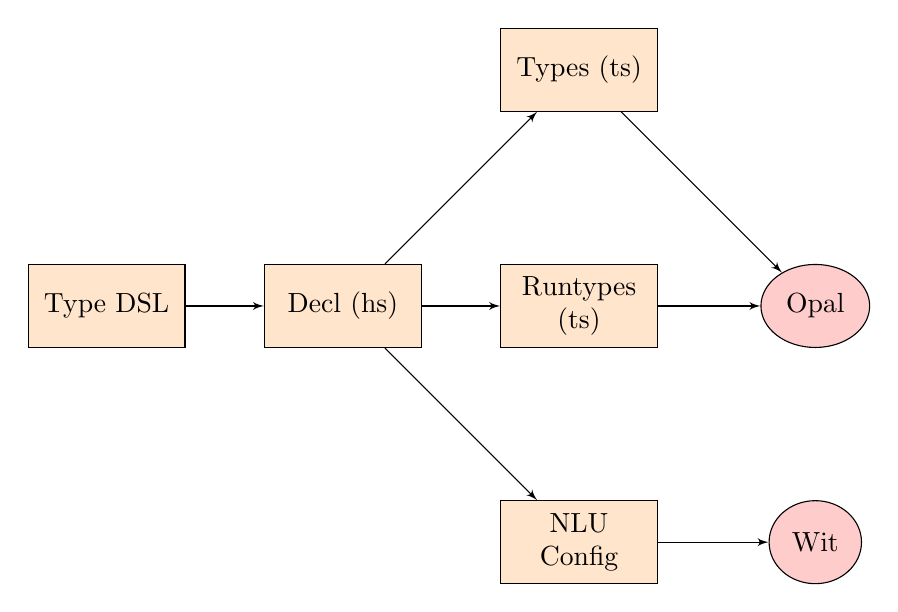
\begin{tikzpicture}[node distance = 3cm, auto]
    \node [block] (types) {Type DSL};
    \node [block, right of=types] (decls_hs) {Decl (hs)};
    \node [block, right of=decls_hs] (decls_ts) {Runtypes (ts)};
    \node [block, below of=decls_ts] (cfg) {NLU Config};
    \node [block, above of=decls_ts] (ts_types) {Types (ts)};
    \node [cloud, right of=decls_ts] (ts) {Opal};
    \node [cloud, right of=cfg] (backend) {Wit};

    \path [line] (types) -- (decls_hs);
    \path [line] (decls_hs) -- (decls_ts);
    \path [line] (decls_hs) -- (cfg);
    \path [line] (decls_hs) -- (ts_types);
    \path [line] (decls_ts) -- (ts);
    \path [line] (ts_types) -- (ts);
    \path [line] (cfg) -- (backend);
  \end{tikzpicture}
  \caption{The configuration process.}
  \label{fig:process}
\end{figure*}

We elected to use a typescript library called \emph{runtypes} to serialize the
AST directly into typescript; this gives us a data structure to guide response
parsing, and also provides us a way to dynamically type-check the results. We
discuss the response parsing algorithm in more detail in section
\ref{implementation}.

Figure \ref{fig:process} shows process of configuring an application for NLU
interaction. The programmer writes types in our DSL, and uses our Haskell tool
to parse the declarations. The tool serializes three artifacts: a set of
Typescript type declarations, a runtypes datastructure, and a set of JSON
configuration files for Wit. The programmer simply imports the types and
runtypes into their Opal project, uploads the JSON files to Wit, and the system
is ready to go.

\section{Formalism} \label{formalism}
In order to reason about the correctness of our translations, we have formalized
the results from section \ref{description}. We begin by formalizing the type DSL
as a pseuo-BNF grammar. This is shown in figure \ref{fig:grammar_a}.
\begin{figure}
  \centering
  \begin{subfigure}{1\linewidth}
    \begin{align*}
      \fcy{D} ::=&\ \text{FreeText}(\etag{t}) \\
      |&\ \text{Keywords}(\etag{t},\ [\ell]) \\
      |&\ \text{Trait}(\etag{t},\ \{s: \fcy{T}\}) \\
      \\
      \fcy{T} ::=&\ \fcy{D} \mid \ell \mid \{s: \fcy{T}\}
    \end{align*}
    $$ \etag{t} \in \textsf{Tag} \qquad \ell, s \in \textbf{string} $$
    \caption{Type DSL}
    \label{fig:grammar_a}
  \end{subfigure}\vspace{1cm}
  \begin{subfigure}{1\linewidth}
    $$ \tau ::=\ \textbf{string} \mid \ell \mid \{s: \tau\} \mid \langle \ell
    \rangle $$
    \caption{Relevant Opal Types}
    \label{fig:grammar_b}
  \end{subfigure}
  \caption{Formal grammars.}
\end{figure}
There are similarities between these definitions and the haskell ones in figure
\ref{fig:ast}, but it has some slightly different goals. First, we remove
aliases and require that all type definitions are written ``in-line''. Next,
rather than split the definition by allowing tags within $\fcy{T}$, we also
require that entitiy definitions are inlined. This means that the data a user
expects from the NLU backend can be represented by a single tree of type
$\fcy{D}$. Importantly, none of these simplifications are fundamental---they
simply remove some aspects of the system that make it easier to use in practice.

In addition to a grammar for the DSL itself, in figure \ref{fig:grammar_b} we
define a grammar of types, $\tau$ which will represent Opal types specifically.
We can think of $\tau$ as representing the final form of the data that a user
hopes to obtain, with no information about the entities that generated the data.
We add a few types that are noteworthy: the type {\bf string} is added to
account for FreeText entities; $\langle {\ell} \rangle$ represents a disjunction
of literals, and covers the case of Keywords entities.

As mentioned above, user's view of their system can be formalized as a top-level
declaration generated by $\fcy{D}$. Since this declaration encompases both type
and configuration information, we would like a way to compute just the
\emph{type} of data that the user expects from the NLU engine. We define the
following mutually recursive functions, which traverse a declaration and
construct a single type in $\tau$.
\begin{align*}
  \text{interp}\ &:\ \fcy{D} \to \tau \\
  \text{interpTy}\ &:\ \fcy{T} \to \tau
\end{align*}

With the basic building blocks defined, we can move forward in formalizing our
system. \fxnote{Should I write out implementations?}

\subsection{Configuration Generation}
The first step that our system takes is configuration. In practice, this is a
two-part process: the user needs to extract the appropriate Opal code as well as
the configuration for the NLU backend. The first step is covered by our
definition of interp. Since we are taking $\tau$ as an analog for relevant Opal
types, the type generation process is exactly the execution of interp on the
top-level entity declaration.

As for the second step, we would like the NLU backend to be set up such that its
responses are \emph{well-formed} with respect to the configuration. Intuitively,
any time we look up some entity tag in the response, we would like to get data
that is compatible with that entity's declaration. We define a type,
\textsf{Resp} of responses, and require that a lookup function exists, with the
following type:
$$ \text{lookup}\ :\ \textsf{Tag} \to \textsf{Resp} \rightharpoonup
\textbf{string} $$
Note that the function is partial; there is no guarantee that the response will
contain the desired data. In the sequel, we will often assume that lookup is
defined on tags we care about, but that assumption will be stated explicitly
rather than assumed by default.

The lookup function always returns a string, but the string might mean any
number of things. The data might be a particular literal, in the case of a
keywords or trait entity, or an entire phrase in the case of a free-text entity.
We define configurations as functions that map a subset of entity tags to the
type of data expected for those entities.
$$ \textsf{Cfg} \equiv \textsf{Tag} \rightharpoonup \tau $$
Now, we call a response well-formed with respect to $\text{cfg} : \textsf{Cfg}$
if and only if it returns appropriate data on lookup. More formally, for some $r
: \textsf{Resp}$,
\begin{align*}
  &r\ \text{well-formed}_{\text{cfg}} \iff \\
  &\forall (\etag{t} : \textsf{Tag}).\ \text{cfg}(\etag{t})\ \text{defined} \Rightarrow \text{lookup}(\etag{t}, r) : \text{cfg(\etag{t})}
\end{align*}

\subsection{Response Parsing}
We discussed above that there is a challenge in parsing the unstructured
response from the NLU engine into data of the appropriate types. This section
will formalize that problem and present our solution.

Our goal will be to write a parsing function which takes a declaration, $d$, and
a response, and produces a value of type interp($d$). We will again write two
mutually recursive functions, parse and parseTy, with types:
\begin{align*}
\text{parse}\ &:\ \Pi_{(d : \fcy{D})}. \textsf{Resp} \rightharpoonup \text{interp}(d) \\
\text{parseTy}\ &:\ \Pi_{(t : \fcy{T})}. \textsf{Resp} \rightharpoonup \text{interp}(t)
\end{align*}
Since we need the type of the result to depend on the declaration, these are
dependent functions. The functions are also partial because lookups might fail.

We will define parse by case analysis on the declaration.
\begin{align*}
  \text{parse}(\text{FreeText}(\etag{t}), r) = \text{lookup}(\etag{t}, r)
\end{align*}
This case is fairly straightforward. Since the interpretation of a free-text
entity is just a string, we can simply look up the value of the appropriate
entity from the response.
\begin{align*}
  \text{parse}(\text{Keywords}(\etag{t}, [\ell_1, \dots, \ell_n]), r) =\\
  \text{lookup}(\etag{t}, r)
\end{align*}
Perhaps surprisingly, we can use the exact same definition in the Keywords case
that we did in the FreeText case. We are required to return a value of type
$\langle {\ell_1 \mid \dots \mid \ell_n} \rangle$; as long as $r$ is
well-formed, it will have been configured to have the same list of literals. We
are guaranteed to get one of them back from lookup.
\begin{align*}
  \text{parse}(\text{Trait}(\etag{t}, rec), r) = \\
  \text{parseTy}(rec[\text{lookup}(\etag{t}, r)], r)
\end{align*}
The final case for parse simply matches the value in the response to an index
into the record, and interprets that record entry using parseTy.

We will not write out the full definition of parseTy, but note that it is fairly
automatic. If the type is another declaration, we can call back to parse, if it
is a literal we simply generate the appropriate string, and if it is a record,
we build the appropriate record and recursively build out its fields.

\subsection{Correctness}
Given a declaration $d$, we generate a configuration, cfg. Then,
\begin{flalign*}
  &\forall\ (r : \textsf{Resp}).\\
  &r\ \text{well-formed}_{\text{cfg}} \Rightarrow \text{parse}(d, r)\ \text{defined}
\end{flalign*}
Note that since parse is a dependent function, it will already return a value of
the correct type. Thus, we only need to care that it is defined. Proof of this
fact is clear by induction on $d$.

\section{Implementation} \label{implementation}

\subsection{Configuration Tool}
When a user wants to configure an Opal application to interact with an NLU
library like Wit, they begin by using our configuration tool. The tool turns
code in the type DSL into typescript code and JSON configuration, and ensures
that the NLU engine responses will agree with the type definitions in the user's
application.

Our configuration tool is written in Haskell, and is designed to be simple and
obviously correct. We use the Parsec library to parse the type DSL into the
intermediate representation mentioned above in figure \ref{fig:ast}.

\subsection{Runtime Library}
At run-time typical application using NLU will go through a fairly consistent
cycle.
\begin{enumerate}
\item Ask user for input, converting voice to text if necessary.
\item Query the NLU engine and obtain a response for the given input.
\item Parse the response into application data.
\item Process parsed data, and repeat.
\end{enumerate}
Steps 1 and 4 are generally application-specific, so we have elected to provide
a library which handles steps 2 and 4. For each backend that Opal
supports,\footnote{At the time of writing, Wit is the only supported backend.}
we provide utilities for querying the API and parsing the response data. The
network code involved in obtaining the response is fairly uninteresting, so we
will focus on the parsing,

In section \ref{formalism}, we outline the parse function, which takes a
declaration and a response and generates an Opal object. The function that we
provide in the Opal library is similar, but there are two important differences.
First, the parse function takes some element of $\fcy{D}$, which it uses to
deduce the structure of the desired output. In the real application, the analog
of $\fcy{D}$ is the \hs{Decl} type in the Haskell code; this is not available to
the Opal application at run time. As mentioned above, we get around this by
using a modified version the runtypes library to keep this information around at
run-time. We extend runtypes to include a type for entities---which map to
declarations in $\fcy{D}$. Runtypes provides the infrastructure for non-entity
types in $\fcy{T}$.

The other difference arises because Opal does not have dependent types. We
cannot completely faithfully transcribe the parse function from above, because
it is not obvious that it can be typed at all. The solution here is to combine
Opal's dynamic typing with runtypes' dynamic checking feature to create a
function that appears to be dependently typed. First, we use dynamic types
within the parse function. While building the response data, we assume, where
necessary, that it has type \ts{any}. Then, once parsing is complete, we use the
runtypes object to check the parsed object, and we cast it to the desired type.
The definition is shown in figure \ref{fig:parse}. The cast is safe, so long as
the user respects the invariant that parse is always called with compatible type
and runtype parameters.

\begin{figure*}
\begin{minted}{typescript}
          public parse<T>(rt: Runtype<any>, res: Response): T {
              return rt.check(this._parse(rt, res)) as T;
          }

          private _parse(rt: Runtype<any>, res: Response): any { ... }
\end{minted}
  \caption{The wit parse functions.}
  \label{fig:parse}
\end{figure*}

\section{Evaluation} \label{evaluation}
%TODO: Cover limitations of the design, possible use-cases, etc

\section{Future Work} \label{future}
Moving forward, we hope to take this work in two main directions---wider support
for NLU features and backends and entirely new features.

\subsection{Wider Support}
Expanding support for more entity types and backends is an obvious way to
increase the usefulness of our work. Here, we discuss both of those extensions
in detail.

\subsubsection{More Types}
In addition to the three ``universal'' kinds of entities (free-text, keywords,
and traits), the Wit NLU engine provides more specialized ways of looking up
entities. Wit provides support for parsing numbers, dates, times, and other
specific forms of text. We elected to keep things simple at first and exclude
these built-in entities, but adding support for them seems like a very
reasonable next-step.

At a first approximation, this would require modifying the definitions of
$\fcy{D}$ and $\tau$ to include declarations for built-in entities and
base types for the data associated with those entities. More work needs to be
done exploring this space before any more specific conclusions can be drawn.

\subsubsection{More Backends}
We are also interested exploring NLU engines beyond Wit. One reason for this is
purely practical---users might want to use other backends, and it would be nice
for Opal to support this. Another reason, however, is more academic. Exploring
other NLU engines would give us opportunities to test the generality of our
current design. Preliminary research suggests that building our type system
around entities and search strategies makes sense, but we can only know that for
sure if we try to build interfaces for more engines.

\subsection{Interesting Features}
There are a number of novel research directions available as extensions to this
project. The following are two of the many ideas that we have had.

\subsubsection{Confidence-Based Parsing}
Up to this point, we have assumed very little about the data returned in the NLU
response. In practice, however, many NLU engines provide more than just
information about the matched entities. Wit, in particular, provides confidence
levels for each entitiy that it finds. Thus, a value like \ts{"Set"} might be
paired with a confidence level of $70\%$, meaning that Wit is $70\%$ sure that
the user's intent is actually to set a new reminder.

As of now, we do not actually use this information. In the majority of cases
that we have tested, a Wit bot either has enough information to get the right
entities, or it does not. However, it is possible that as we attempt to support
new types of entities and as user types get more complicated, it will be useful
to try multiple parses of a single response. In that case, we can choose between
different parses using confidence scores.

\subsubsection{Training with Tests}
A final extension of this project would attempt to close the code/configuration
gap even further by allowing users to train their NLU application in a way that
is guaranteed to support their tests. We would accomplish this using the same
idea behind our type DSL---we introduce a new DSL (or an extension to the
current one) for generating both Wit training examples and application tests.
While synchronization is less of an issue with training than it is with
configuration, it would still be extremely convenient to express the entirety of
the application's behavior in one place.

Exploring this path would require a fair amount of implementation work, but we
would also need to take great care to avoid overfitting. It is unclear to what
extent this would become an issue.

\section{Conclusion} \label{conclusion}
% TODO: Write

\end{document}